% =====================================================================
% stats.tex: supplement text for effect size, detection-n, equivalence, the
% noise-floor audit and the kernel analysis. Five blocks, each headed by
% the place it goes in sec/X_appendix.tex. Source runs:
%   outputs/run_20261108_205428_stats_fixes  (results.json: effects, effects2,
%     floor_sim, floor_audit, kernel, gates_recheck; notes §88, results T115)
%   outputs/run_20261109_152704_rankflips_functional_rebase/fig_detection.py
%     (the figure, from the same effects.detection_n block)
% =====================================================================


% =====================================================================
% BLOCK A. Effect size.
% EXTENDS \subsection{Reading a squared statistic over a population of prompts}
% (\label{app:failrate}): append after its last paragraph ("One caution on the
% readout ..."). Nothing in that subsection is replaced.
% =====================================================================
\paragraph{An effect size for comparing metrics.} A separation in noise floors is a test
statistic: it grows linearly in $n$ (Sec.~\ref{app:nscale}) and at a different rate per
metric, so a ratio of two metrics' separations is not a ratio of what they see. The readout
above gives a quantity that does not grow with $n$,
$e = \sqrt{\mathrm{MMD}^2_{\text{arm}}}\,/\,\sqrt{\mathrm{MMD}^2_{\randomvox{}}}$ under the
same metric, which reads $0$ for real data and $1$ for the anchor whatever the metric.
Table~\ref{tab:effect} gives it for every probe at $n{=}256$. The two interior probes sit at
$0.03$ and $0.02$ of the anchor on appearance, inside the $95$th percentile of fresh real
draws ($0.031$), and at $0.78$ and $0.60$ on geometry. \matshuffle{} and \monochrome{} are
the converse. \patchstitch{} sits as far from real on geometry as on appearance, so its
near-real local statistics buy it no geometric advantage. Read between a probe and its own
source builds, the render features of \solidify{} do move, by $0.018$ $[0.014, 0.024]$ of the
anchor against a paired null of $0.005$: that is the glass leak of Sec.~\ref{app:hull}, $44$
times smaller than \vkid{}'s $0.80$ on the same pairs.

\begin{table}[h]
\centering
\small
\setlength{\tabcolsep}{3pt}
\caption{\textbf{Effect size} $e$, $\sqrt{\mathrm{MMD}^2}$ over that of \randomvox{} under
the same metric, $n{=}256$ against the $399$-build reference, with half-sampling $95\%$
intervals. The $95$th percentile of fresh real draws is $0.031$ (\mvkid{}) and $0$
(\vkid{}). BrickGPT is scored on the LEGO suite, where the anchor is \singlemode{}.}
\label{tab:effect}
\begin{tabular}{lccr}
\toprule
arm & \mvkid{} & \vkid{} & ratio \\
\midrule
\solidify{}     & $0.03$ {\scriptsize$[0.00, 0.08]$} & $0.78$ {\scriptsize$[0.74, 0.83]$} & $27$ \\
\hollow{}       & $0.02$ {\scriptsize$[0.00, 0.08]$} & $0.60$ {\scriptsize$[0.57, 0.63]$} & $26$ \\
\growshell{}    & $0.47$ {\scriptsize$[0.44, 0.50]$} & $0.80$ {\scriptsize$[0.77, 0.84]$} & $1.7$ \\
\matshuffle{}   & $0.62$ {\scriptsize$[0.60, 0.65]$} & $0$                                & $0$ \\
\monochrome{}   & $0.70$ {\scriptsize$[0.68, 0.73]$} & $0$                                & $0$ \\
\patchstitch{}  & $0.63$ {\scriptsize$[0.61, 0.66]$} & $0.71$ {\scriptsize$[0.69, 0.73]$} & $1.1$ \\
BrickGPT        & $0.17$                             & $0.37$                             & $2.2$ \\
\bottomrule
\end{tabular}
\end{table}


% =====================================================================
% BLOCK B. Detection-n and equivalence.
% EXTENDS \subsection{The head-to-head test} (\label{app:significance}): append
% after its second paragraph ("Recomputing the run of record ..."). Nothing in
% that subsection is replaced; its p from 0.61 to 0.77 is the n=128 protocol
% run, the 0.87 below is the n=256 leaderboard draw.
% Figure file: drafts_20261109/fig_detection.pdf -> figures/fig_detection.pdf
% =====================================================================
\paragraph{Non-detection, and equivalence.} Every probe is built from the same builds as the
real arm it is compared with. The label-permutation test treats the two arms as independent,
which is exact under its null but discards the pairing, so on a probe it is conservative:
\solidify{} against real reads $p{=}0.87$ at $n{=}256$. A paired test that swaps labels
within each build and its probe reads $p{=}0.055$ for the same $+0.35$ floors, and $0.82$ for
\hollow{}. Across $n$ from $8$ to $256$ the paired test never reaches $80\%$ power on either
interior probe under \mvkid{} (at most $0.20$), while \vkid{} detects both at $n{=}8$
(Fig.~\ref{fig:detection}). Non-rejection is not equivalence, so we also test equivalence
against a margin fixed in advance, two noise floors, with two one-sided tests whose standard
error is that of a fresh draw of $256$ builds and of the reference, from the Hoeffding
decomposition of the paired difference. \solidify{} reads $+0.35$ floors with $90\%$
interval $[-0.28, +0.98]$ and \hollow{} $+0.04$ with $[-0.25, +0.33]$, both equivalent to real
($p{<}0.001$); the same holds for a margin of $0.05$ in effect size ($\pm 2.7$ floors). Under
\vkid{} neither is equivalent, at $444$ and $265$ floors.

\begin{figure*}[t]
\centering
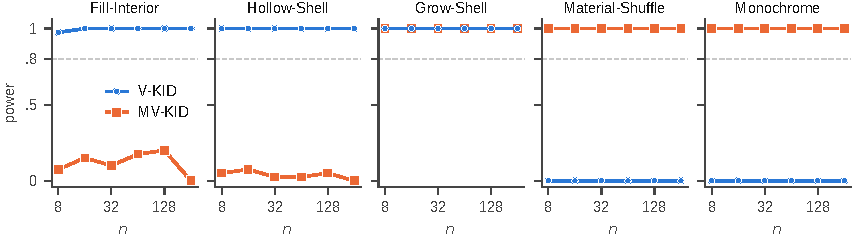
\includegraphics[width=\linewidth]{figures/fig_detection}
\caption{\textbf{Detection as a function of $n$.} Power of the paired permutation test
($\alpha{=}0.05$, $999$ permutations) of each probe against its own source builds, over $40$
random subsets per $n$ below $256$ and the full set at $n{=}256$; dashed line, $80\%$.
\vkid{} detects \solidify{}, \hollow{} and \growshell{} at $n{=}8$. \mvkid{} detects
\growshell{}, \matshuffle{} and \monochrome{} at $n{=}8$ and never reaches $80\%$ power on
\solidify{} or \hollow{}.}
\label{fig:detection}
\end{figure*}


% =====================================================================
% BLOCK C. Noise-floor audit.
% REPLACES the last four sentences of \subsection{The $n{=}256$ leaderboard and
% the $n{=}128$ protocol run} (\label{app:n256}), from "The noise floor at
% $n{=}256$ is estimated from $256$ of the $399$ test builds per draw" to
% "The ranks do not depend on it." The rank-interval sentences before them stay.
% Also EXTENDS \paragraph{The unit is itself estimated.} in app:nscale: no edit
% needed there, the last two sentences below cite its 10% figure.
% =====================================================================
\paragraph{Calibrating the finite-population correction.} The floor at $n{=}256$ draws
$256$ of the $399$ test builds per replicate and divides the spread of those overlapping
draws by $\sqrt{1-n/N}$. For a degenerate U-statistic the leading variance term carries
$(1-f)^2$ rather than $(1-f)$, which would make this correction too small, but the pool's own
kernel matrix adds a first-order term of order $\zeta_2/N$ that more than offsets it. We
measure the net effect against non-overlapping draws: a reference of $399$ and a population
of $1{,}464$ real builds, both drawn from the training split so that the statistic sits in the
same near-degenerate regime, with the true spread read off disjoint $n$-sets of the
population. The true spread is $0.88$ to $0.95$ of the bench floor at $n{=}256$ and $0.89$ to
$0.93$ at $n{=}128$, for both metrics, so the floor is slightly conservative; a $(1-f)$
correction would overstate it by a factor near $1.8$. On the leaderboard's own pool an
unbiased Hoeffding estimate, accurate to $5\%$ in the simulation, puts the stored \vkid{}
floor $11\%$ above the true one and the stored \mvkid{} floor $2.5\%$ below it. The larger
term is the Monte-Carlo error of Sec.~\ref{app:nscale}: $48$ draws pin the \vkid{} floor at
$n{=}256$ only to $[0.043, 0.067]$ at $95\%$, which is why two runs scoring the same raw
distance against two $48$-draw floors can read \matshuffle{} at $+422$ and at $+346$. We keep
each run's stored floor; under the corrected floor no gate verdict of \vkid{} or \mvkid{}
changes and no ranking changes.


% =====================================================================
% BLOCK D. Kernel and preprocessing.
% NEW \subsection, placed last in \section{Robustness of \vkid{}}
% (\label{app:vkid-robust}), i.e. after % Source: outputs/run_20261106_193358_vkid_robustness (notes §82, results T105).
\subsection{Families, random subsets and generic descriptors}

Each test below runs under the bench's own scoring code: the blocking gates on the ladder
($n{=}128$, $48$ fresh real draws, geometry rungs) and the separations on the $n{=}256$
leaderboard of record, whose build hashes we verify. Every row is whitened on the reference
and scored by the same unbiased KID, and every separation is in that row's own noise floor.
Rank agreement is Spearman's $\rho$ over the nine structural arms of the board against full
\vkid{}.

\paragraph{No family carries the result.}
We group the $77$ dimensions into seven families: $55$ pattern orbits, thickness ($5$
bins and $2$ scalars), height ($8$ bins and the entropy), surface ($2$), symmetry ($1$),
interior ($2$) and size ($1$). Removing any one family keeps every gate passing,
\solidify{} between $310$ and $457$ floors (full $444.4$), \hollow{} between $146$ and
$270$ (full $265.4$), and $\rho \geq 0.95$ (Table~\ref{tab:vkid-robust}). Random subsets
tell the same story without any grouping of ours: $20$ of $20$ random $38$-dimensional
subsets pass every gate, with \solidify{} at a median of $351$ floors (minimum $283$),
\hollow{} at $221$ ($133$) and $\rho$ at $0.97$ ($0.88$). At $19$ dimensions, $17$ of $20$
pass, and the weakest still separates \solidify{} by $179$ floors.

\paragraph{A descriptor with no hand design passes.}
We replace the descriptor by generic maps $\phi$ of the occupancy grid, made exactly
invariant to the yaw group by orbit averaging, $f(x) = \tfrac{1}{8}\sum_{g \in D_4}
\phi(gx)$, which is the only design step they share. Three are random-weight
three-layer 3D CNNs with mean and max pooling per layer ($224$ dimensions, three weight
draws), one is a feature-hashed histogram of raw $3^3$ occupancy patterns ($256$), and one
counts occupied $3^3$ neighbours of solid and air cells at $1\times$, $2\times$ and
$4\times$ pooling ($168$). All six rows, including the concatenation of a CNN with the
counts, pass every gate and separate \solidify{} by $257$ to $437$ floors and \hollow{} by
$166$ to $297$. Occupancy KID on a centred, pooled grid fails noise ordering and
invariance (Sec.~\ref{app:headtohead}); orbit averaging is what turns the raw volume into
a valid metric, and the separation follows from observing the volume rather than from
the choice of features. The generic rows reproduce \vkid{}'s ordering of probes and
baselines ($\rho$ between $0.8$ and $1.0$ over five arms) and differ from it in the
order of the four learned arms, where the random CNNs place Dream-Cubed behind the three
autoregressive arms; we report \vkid{} as the instantiation, and the ordering of close
learned arms as descriptor-dependent.

\paragraph{Global coherence is a separate axis.}
\patchstitch{} tiles $8^3$ patches of different real builds, so it is the natural attack
on a local descriptor. \vkid{} places it $368.2$ floors from real, fourth of nine arms.
Appending global terms, the largest 26-connected part ratio and component count, or
$2^3$ orbit histograms of the $2\times$ and $4\times$ max-pooled grid, keeps every gate
and leaves it fourth, with its separation between $0.73$ and $0.81$ of \solidify{}'s
($0.83$ for \vkid{}). The connected-part ratio on its own separates \patchstitch{} by
$258$ floors and both interior probes by none, so coherence is measurable and orthogonal
to the interior axis; at two of $79$ dimensions it does not move the joint kernel. We
keep \vkid{} unchanged and state its scope as local geometry.

\begin{table}[t]
\centering
\small
\caption{\vkid{} robustness. Gates on the ladder ($n{=}128$); separations on the
$n{=}256$ board in each row's own noise floor; $\rho$: Spearman over nine arms against
full \vkid{}. Random rows give the median and, in brackets, the minimum over $20$ draws.}
\label{tab:vkid-robust}
\setlength{\tabcolsep}{3pt}
\resizebox{\linewidth}{!}{%
\begin{tabular}{lrcrrrr}
\toprule
descriptor & dims & gates & \solidify{} & \hollow{} & \patchstitch{} & $\rho$ \\
\midrule
full \vkid{}                    & $77$  & pass & $444.4$ & $265.4$ & $368.2$ & $1.00$ \\
\midrule
\multicolumn{7}{l}{\emph{leave one family out}} \\
without pattern orbits          & $22$  & pass & $457.4$ & $146.0$ & $342.1$ & $1.00$ \\
without thickness               & $70$  & pass & $310.4$ & $265.8$ & $374.4$ & $0.95$ \\
without height                  & $68$  & pass & $414.0$ & $251.4$ & $342.7$ & $1.00$ \\
without surface                 & $75$  & pass & $441.8$ & $258.3$ & $360.9$ & $1.00$ \\
without symmetry                & $76$  & pass & $451.1$ & $270.3$ & $357.7$ & $1.00$ \\
without interior                & $75$  & pass & $421.8$ & $258.7$ & $327.0$ & $1.00$ \\
without size                    & $76$  & pass & $440.9$ & $263.8$ & $374.6$ & $1.00$ \\
\midrule
\multicolumn{7}{l}{\emph{random subsets, 20 draws}} \\
$50\%$                          & $38$  & $20/20$ & $351\,[283]$ & $221\,[133]$ & $317\,[230]$ & $0.97\,[0.88]$ \\
$25\%$                          & $19$  & $17/20$ & $298\,[179]$ & $153\,[56]$  & $246\,[178]$ & $0.95\,[0.85]$ \\
\midrule
\multicolumn{7}{l}{\emph{no hand design, orbit-averaged}} \\
random 3D CNN, draw 1           & $224$ & pass & $339.4$ & $223.8$ & $277.8$ & $0.80$ \\
random 3D CNN, draw 2           & $224$ & pass & $437.3$ & $297.4$ & $284.7$ & $0.73$ \\
random 3D CNN, draw 3           & $224$ & pass & $403.6$ & $242.1$ & $309.5$ & $0.80$ \\
hashed $3^3$ patterns           & $256$ & pass & $256.7$ & $208.9$ & $326.0$ & $0.75$ \\
multi-scale neighbour counts    & $168$ & pass & $359.3$ & $166.3$ & $514.9$ & $0.80$ \\
random 3D CNN + counts          & $392$ & pass & $396.4$ & $230.7$ & $406.1$ & $0.78$ \\
\midrule
\multicolumn{7}{l}{\emph{global terms}} \\
\vkid{} + connected parts       & $79$  & pass & $454.6$ & $271.4$ & $366.1$ & $1.00$ \\
\vkid{} + pooled orbits         & $187$ & pass & $485.3$ & $253.4$ & $354.1$ & $1.00$ \\
connected parts alone           & $2$   & pass & $0.0$   & $0.1$   & $258.4$ & $-0.20$ \\
\bottomrule
\end{tabular}}
\end{table}
 and before
% the fig:nn figure. Optional one-line pointer at the end of
% \paragraph{Estimator and kernel.} in Sec. A:
%   "Sec.~\ref{app:kernel} shows that no conclusion depends on this kernel."
% =====================================================================
\subsection{Kernel and preprocessing}
\label{app:kernel}

With unit-norm rows and $t = a^{\top}b/D \in [-1/D, 1/D]$, the cubic kernel expands as
$(1+t)^3 = 1 + 3t + 3t^2 + t^3$. On every probe the linear term carries $99.8\%$ of \mvkid{}
and $98.8$ to $99.5\%$ of \vkid{}, so both metrics are in effect tests of a difference in mean
embedding; differences in spread, such as mode collapse, are left to the diversity and
memorization gates. Table~\ref{tab:kernel} varies the kernel and the preprocessing. Every
\vkid{} variant leaves \solidify{} and \hollow{} hundreds of floors from real, scores
\matshuffle{} at exactly $0$ and passes every gate of the geometry ladder at $n{=}64$ and
$128$. Whitening and the clip set the magnitudes: removing the clip lowers \solidify{} from
$422$ to $288$ floors, and removing whitening raises it to $1{,}637$ while lowering
\growshell{} to $165$. On the render side, whitening the DINOv2 features against the
reference leaves \solidify{} at $0.50$ floors and \hollow{} at $0.06$.

\begin{table}[h]
\centering
\small
\setlength{\tabcolsep}{3.5pt}
\caption{\textbf{Kernel and preprocessing ablation.} Separations in each variant's own noise
floor (the bench estimator's expected value, so the base \vkid{} row reads $422$ where the
card's $48$-draw floor gives $444$), $n{=}256$, $399$-build reference. Gates: the geometry
ladder at $n{=}64$ and $128$; $^\ast$the render ladder at $n{=}64$.}
\label{tab:kernel}
\resizebox{\linewidth}{!}{%
\begin{tabular}{lrrrrl}
\toprule
variant & \solidify{} & \hollow{} & \growshell{} & \matshuffle{} & gates \\
\midrule
\vkid{}, cubic          & $422$     & $252$  & $446$ & $0$   & pass \\
\quad linear kernel     & $419$     & $251$  & $444$ & $0$   & pass \\
\quad RBF, median       & $475$     & $266$  & $485$ & $0$   & pass \\
\quad no clip           & $288$     & $247$  & $409$ & $0$   & pass \\
\quad no whitening      & $1{,}637$ & $213$  & $165$ & $0$   & pass \\
\quad no whitening, RBF & $692$     & $160$  & $180$ & $0$   & pass \\
\midrule
\mvkid{}, cubic         & $0.31$    & $0.03$ & $206$ & $365$ & pass$^\ast$ \\
\quad linear kernel     & $0.31$    & $0.03$ & $206$ & $365$ & --- \\
\quad RBF, median       & $0.32$    & $0.03$ & $215$ & $351$ & pass$^\ast$ \\
\quad whitened DINOv2   & $0.50$    & $0.06$ & $200$ & $277$ & --- \\
\bottomrule
\end{tabular}}
\end{table}
